\documentclass[dvipdfm]{beamer}
\usepackage{stysty}

\usetheme{Rochester}

\setbeamertemplate{footline}[frame number]
\AtBeginSection[]{
    \frame{\tableofcontents[currentsection, hideallsubsections]} %目次スライド
}

\title{たしざん・かけざんだけでまなぶりょーしりきがく}
\author{低音}

\begin{document}

\begin{frame}
    \titlepage
\end{frame}

\begin{frame}{自己紹介}
\end{frame}

\begin{frame}{このセミナーで登場しないもの}
    \begin{itemize}
        \item 実験事実
        \item 波動関数
        \item シュレディンガー方程式
        \item 微積分
        \item 三角関数
    \end{itemize}
\end{frame}

\begin{frame}{なぜ「物理」をやらないのか?}
    \begin{enumerate}
        \item 現象が\alert{\textbf{直観とかけ離れている}}
        \begin{itemize}
            \item 状態の重ね合わせ?
            \item 測定したら状態が変わる?
            \item 位置と速度が同時に決まらない?
            \item 量子もつれ?
        \end{itemize}
        \item \alert{\textbf{学部1年の線形代数だけ}}で理解できる
        \begin{itemize}
            \item 複素ベクトル
            \item エルミート行列
            \item ユニタリ行列
        \end{itemize}
    \end{enumerate}
    \textbf{計算できるようになると、なぜか感覚を掴めてくる}
\end{frame}



\section{べくとるとぎょーれつ}

\subsection{たしざん・かけざんのふくしゅう}


\subsection{べくとる}

\begin{frame}{ベクトル}
    ベクトルは数がいっぱい並んだもの。
    4つ数が並ぶと4次元。

    量子力学のお約束に従って、ブラ・ケットで書くと、後々直感的にわかりやすい。
    \begin{equation*}
        \ket{1,2,4,3}
        =
        \mqty[1\\2\\4\\3]
        =
        \vcenter{\hbox{
            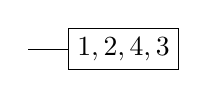
\begin{tikzpicture}
                \node at(0,0)[draw,rectangle](ket){$\ket{1,2,4,3}$};
                \draw(ket.west)--++(-.5,0);
            \end{tikzpicture}
        }}
    \end{equation*}
    \begin{equation*}
        \bra{1,2,4,3}
        =
        \mqty[1&2&4&3]
        =
        \vcenter{\hbox{
            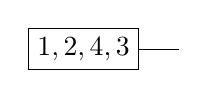
\begin{tikzpicture}
                \node at(0,0)[draw,rectangle](ket){$\bra{1,2,4,3}$};
                \draw(ket.east)--++(.5,0);
            \end{tikzpicture}
        }}
    \end{equation*}
    量子力学ではベクトルは状態を表すので、\alert{\textbf{状態ベクトル}}と呼ぶことにする。
\end{frame}

\begin{frame}{状態ベクトルの足し算}
    同じ次元のブラ同士、ケット同士なら単純に足すだけ。
    \begin{equation*}
        \mqty[1\\2\\4\\3]
        +
        \mqty[5\\3\\1\\4]
        =
        \mqty[6\\5\\5\\7]
    \end{equation*}
    次元が違うもの、ブラとケットは足せない。

    足し算の延長でスカラー倍もそのまま。
    \begin{equation*}
        3\mqty[1\\2\\4\\3]
        =
        \mqty[3\\6\\12\\9]
    \end{equation*}
\end{frame}

\begin{frame}{状態ベクトルどうしの掛け算 (内積)}
    \begin{equation*}
        \begin{split}
            \mqty[\red{1} & \blue{2} & \green{4} & 3]
            \mqty[\red{5} \\ \blue{1} \\ \green{-3}\\ 2]
            &=
            \red{1\cdot5}
            +
            \blue{2\cdot1}
            +
            \green{4\cdot(-3)}
            +
            3\cdot2
            \\
            &=
            1
        \end{split}
    \end{equation*}
    具体的な計算をしないなら、お絵描きしたほうがわかりやすい。
    \begin{equation*}
        \vcenter{\hbox{
            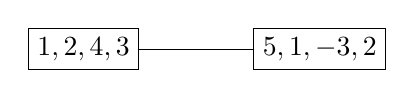
\begin{tikzpicture}
                \node at(0,0)[draw,rectangle](ket){$\ket{5,1,-3,2}$};
                \node at(-3,0)[draw,rectangle](bra){$\bra{1,2,4,3}$};
                \draw(bra.east)--(ket.west);
            \end{tikzpicture}
        }}
        =
        1
    \end{equation*}
    脚が出てないので状態ベクトルじゃない。
\end{frame}


\subsection{たしざん・かけざんがいっぱい}

\begin{frame}{一方その頃量子力学では}
    量子力学では, すべての情報はベクトルが持っている.

    状態ベクトル=状態。
    \begin{prop*}{測定により$\ket{\psi}$が測定される確率}{}
        \begin{equation*}
            P_\psi
            \propto
            \braket{\psi}
            =
            \vcenter{\hbox{
                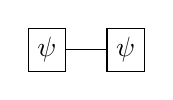
\begin{tikzpicture}
                    \node at(0,0)[draw,rectangle](ket){$\ket{\psi}$};
                    \node at(-1,0)[draw,rectangle](bra){$\bra{\psi}$};
                    \draw(bra.east)--(ket.west);
                \end{tikzpicture}
            }}
        \end{equation*}
    \end{prop*}

    状態って???

    $\rightarrow$詳しい話はこの後
\end{frame}

\begin{frame}{行列の状態ベクトルへの作用}
    \begin{equation*}
        \mqty[\red{1} & \blue{2} \\ \green{-1} & \purple{4}]
        \mqty[1 \\ -2]
        =
        \mqty[
            \red{1}\cdot1+\blue{2}\cdot(-2)
            \\
            \green{-1}\cdot1+\purple{4}\cdot(-2)
        ]
        =
        \mqty[-3\\-9]
    \end{equation*}
    こういうのを
    \begin{equation*}
        \hat{H}\ket{\psi}
        =
        \ket{H\psi}
    \end{equation*}
    \begin{equation*}
        \vcenter{\hbox{
            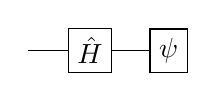
\begin{tikzpicture}
                \node at(0,0)[draw, rectangle](H){$\hat{H}$};
                \node at(1,0)[draw, rectangle](psi){$\ket{\psi}$};
                \draw(H.east)--(psi.west)(H.west)--++(-.5,0);
            \end{tikzpicture}
        }}
        =
        \vcenter{\hbox{
            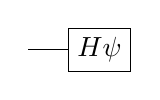
\begin{tikzpicture}
                \node at(1,0)[draw, rectangle](psi){$\ket{H\psi}$};
                \draw(psi.west)--++(-.5,0);
            \end{tikzpicture}
        }}
    \end{equation*}
    みたいに書く。
    $\hat{H}$は状態ベクトルを状態ベクトルにするので脚が2本。
    \begin{equation*}
        \hat{H}
        =
        \vcenter{\hbox{
            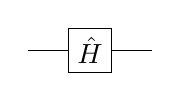
\begin{tikzpicture}
                \node at(0,0)[draw,rectangle](H){$\hat{H}$};
                \draw(H.east)--++(.5,0);
                \draw(H.west)--++(-.5,0);
            \end{tikzpicture}
        }}
    \end{equation*}
\end{frame}

\begin{frame}{行列積}
    \begin{equation*}
        \begin{split}
            &
            \mqty[
                a & b
                \\
                c & d
            ]
            \mqty[
                e & f
                \\
                g & h
            ]
            \mqty[\alpha \\ \beta]
            =
            \mqty[
                a & b
                \\
                c & d
            ]
            \mqty[
                e\alpha+f\beta
                \\
                g\alpha+h\beta
            ]
            \\
            &=
            \mqty[
                a(e\alpha+f\beta)+b(g\alpha+h\beta)
                \\
                c(e\alpha+f\beta)+d(g\alpha+h\beta)
            ]
            \\
            &=
            \mqty[
                (ae+bg)\alpha+(af+bh)\beta
                \\
                (ce+dg)\alpha+(cf+dh)\beta
            ]
            \\
            &=
            \mqty[
                ae+bg & af+bh
                \\
                ce+dg & cf+dh
            ]
            \mqty[\alpha \\ \beta]
        \end{split}
    \end{equation*}
    \begin{equation*}
        \mqty[
            a & b
            \\
            c & d
        ]
        \mqty[
            e & f
            \\
            g & h
        ]
        =
        \mqty[
            ae+bg & af+bh
            \\
            ce+dg & cf+dh
        ]
    \end{equation*}
    \begin{equation*}
        \vcenter{\hbox{
            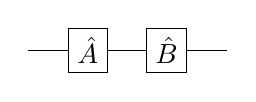
\begin{tikzpicture}
                \node at(0,0)[draw,rectangle](A){$\hat{A}$};
                \node at(1,0)[draw,rectangle](B){$\hat{B}$};
                \draw(A.east)--(B.west);
                \draw(A.west)--++(-.5,0);
                \draw(B.east)--++(.5,0);
            \end{tikzpicture}
        }}
        =
        \vcenter{\hbox{
            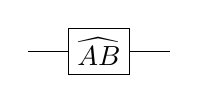
\begin{tikzpicture}
                \node at(0,0)[draw,rectangle](A){$\widehat{AB}$};
                \draw(A.west)--++(-.5,0);
                \draw(A.east)--++(.5,0);
            \end{tikzpicture}
        }}
    \end{equation*}
\end{frame}

\begin{frame}{行列積}
    \begin{equation*}
        \begin{split}
            &
            \mqty[
                A_{11} & A_{12} & \cdots & A_{1N}
                \\
                A_{\red{2}1} & A_{\red{2}2} & \cdots & A_{\red{2}N}
                \\
                \vdots & \vdots & \ddots & \vdots
                \\
                A_{N1} & A_{N2} & \cdots & A_{NN}
            ]
            \mqty[
                B_{1\blue{1}} & B_{12} & \cdots & B_{1N}
                \\
                B_{2\blue{1}} & B_{22} & \cdots & B_{2N}
                \\
                \vdots & \vdots & \ddots & \vdots
                \\
                B_{N\blue{1}} & B_{N2} & \cdots & B_{NN}
            ]
            \\
            &=
            \mqty[
                A_{11}B_{11}+\cdots+A_{1N}B_{N1} & \cdots & A_{11}B_{1N}+\cdots+A_{1N}B_{NN}
                \\
                A_{\red{2}1}B_{1\blue{1}}+\cdots+A_{\red{2}N}B_{N\blue{1}} & \cdots & A_{21}B_{1N}+\cdots+A_{2N}B_{NN}
                \\
                \vdots & \ddots & \vdots
                \\
                A_{N1}B_{11}+\cdots+A_{NN}B_{N1} & \cdots & A_{N1}B_{1N}+\cdots+A_{NN}B_{NN}
            ]
        \end{split}
    \end{equation*}
    \begin{equation*}
        (AB)_{\red{i}\blue{j}}
        =
        A_{\red{i}1}B_{1\blue{j}}+\cdots+A_{\red{i}N}B_{N\blue{j}}
    \end{equation*}

    むずそうなことやってるけど、結局は足し算と掛け算がいっぱいあるだけ。
\end{frame}


\subsection{量子力学との関係}

\begin{frame}{一方その頃量子力学では}
    状態を変換すると別の状態になる
    \begin{itemize}
        \item 回転する
        \item ズラす
        \item 交換する
    \end{itemize}
    状態ベクトルを状態ベクトルに移すので、行列による作用で表せる
    \begin{equation*}
        \vcenter{\hbox{
            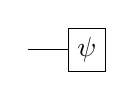
\begin{tikzpicture}
                \node at(1,0)[draw, rectangle](psi){$\ket{\psi}$};
                \draw(psi.west)--++(-.5,0);
            \end{tikzpicture}
        }}
        \mapsto
        \vcenter{\hbox{
            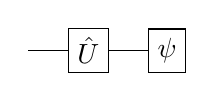
\begin{tikzpicture}
                \node at(0,0)[draw, rectangle](H){$\hat{U}$};
                \node at(1,0)[draw, rectangle](psi){$\ket{\psi}$};
                \draw(H.east)--(psi.west)(H.west)--++(-.5,0);
            \end{tikzpicture}
        }}
    \end{equation*}
\end{frame}


\section{こゆーほーてーしき}

\begin{frame}{わかる人には一発でわからせる固有方程式}
    \begin{dfn}{固有方程式}{}
        \begin{equation*}
            \mqty[
                H_{11} & \cdots & H_{1N}
                \\
                \vdots & \ddots & \vdots
                \\
                H_{N1} & \cdots & H_{NN}
            ]
            \underset{\red{\text{固有状態ベクトル}}}{
                \mqty[
                    \phi_1 \\ \vdots \\ \phi_N
                ]
            }
            =
            \underset{\red{\text{固有値}}}{E}
            \underset{\red{\text{固有状態ベクトル}}}{
                \mqty[
                    \phi_1 \\ \vdots \\ \phi_N
                ]
            }
        \end{equation*}
        \begin{equation*}
            \hat{H}\ket{\phi}
            =
            E\ket{\phi}
        \end{equation*}
        \begin{equation*}
            \vcenter{\hbox{
                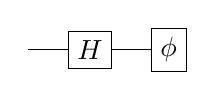
\begin{tikzpicture}
                    \node at(-1,0)[draw,rectangle](H){$H$};
                    \node at(0,0)[draw,rectangle](psi){$\ket{\phi}$};
                    \draw(H.east)--(psi.west)(H.west)--++(-.5,0);
                \end{tikzpicture}
            }}
            =
            E
            \vcenter{\hbox{
                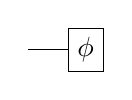
\begin{tikzpicture}
                    \node at(0,0)[draw,rectangle](psi){$\ket{\phi}$};
                    \draw(psi.west)--++(-.5,0);
                \end{tikzpicture}
            }}
        \end{equation*}
    \end{dfn}
\end{frame}

\begin{frame}{固有方程式 定義のポイント}
    \begin{equation*}
        \vcenter{\hbox{
            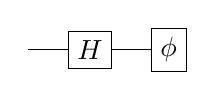
\begin{tikzpicture}
                \node at(-1,0)[draw,rectangle](H){$H$};
                \node at(0,0)[draw,rectangle](psi){$\ket{\phi}$};
                \draw(H.east)--(psi.west)(H.west)--++(-.5,0);
            \end{tikzpicture}
        }}
        =
        E
        \vcenter{\hbox{
            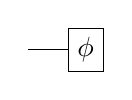
\begin{tikzpicture}
                \node at(0,0)[draw,rectangle](psi){$\ket{\phi}$};
                \draw(psi.west)--++(-.5,0);
            \end{tikzpicture}
        }}
    \end{equation*}
    \begin{itemize}
        \item 両辺の固有状態ベクトル$\ket{\phi}$は同じ
        \item 固有値$E$はただの実数
    \end{itemize}
    $H$を決めると$(E, \ket{\phi})$の組が (一般には複数個) 出現
\end{frame}

\begin{frame}{例}
    \begin{equation*}
        \hat{H}
        =
        \mqty[
            1 & 0
            \\
            0 & -1
        ]
        \Longrightarrow
        (E,\ket{\phi})
        =
        \qty(1,\mqty[1\\0]),
        \qty(-1,\mqty[0\\1])
    \end{equation*}
    \begin{equation*}
        \hat{H}
        =
        \mqty[
            0 & 1
            \\
            1 & 0
        ]
        \Longrightarrow
        (E,\ket{\phi})
        =
        \qty(1,\mqty[1/\sqrt{2}\\1/\sqrt{2}]),
        \qty(1,\mqty[1/\sqrt{2}\\-1/\sqrt{2}])
    \end{equation*}
\end{frame}

\begin{frame}{手を動かせ}
    \begin{eg*}{$2\times2$でやってみよう!}{}
        \begin{equation*}
            \mqty[0 & 1 \\ 1 & 0]
            \mqty[1 \\ 1]
            =
            \mqty[0\cdot1+1\cdot1 \\ 1\cdot1+0\cdot1]
            =
            \mqty[1 \\ 1]
        \end{equation*}
        \begin{equation*}
            \mqty[0 & 1 \\ 1 & 0]
            \mqty[1 \\ -1]
            =
            \mqty[0\cdot1+1\cdot(-1) \\ 1\cdot1+0\cdot(-1)]
            =
            -\mqty[1 \\ -1]
        \end{equation*}
    \end{eg*}
    一般に行列$\hat{H}$から固有値$E$と固有状態ベクトル$\ket{\phi}$を見つけるのは至難の業
    (原理的にはできるが計算が膨大)。
\end{frame}

\begin{frame}{期待値ってなに?}
    \begin{equation*}
        \ev{\hat{H}}{\psi}
        =
        \vcenter{\hbox{
            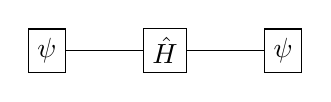
\begin{tikzpicture}
                \node at(0,0)[draw, rectangle](H){$\hat{H}$};
                \node at(1.5,0)[draw, rectangle](ket){$\ket{\psi}$};
                \node at(-1.5,0)[draw, rectangle](bra){$\bra{\psi}$};
                \draw(H.west)--(bra.east);
                \draw(H.east)--(ket.west);
            \end{tikzpicture}
        }}
    \end{equation*}
    期待値に見える?

    → 固有状態ベクトルに直せばわかる!
\end{frame}

\begin{frame}{固有方程式で見る期待値}
    $\hat{H}$の固有値$E_1,E_2,\dots$の固有ベクトル$\ket{E_1},\ket{E_2},\dots$により
    \begin{equation*}
        \vcenter{\hbox{
            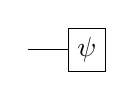
\begin{tikzpicture}
                \node at(1.5,0)[draw, rectangle](ket){$\ket{\psi}$};
                \draw(ket.west)--++(-.5,0);
            \end{tikzpicture}
        }}
        =
        c_1
        \vcenter{\hbox{
            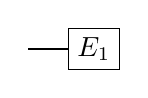
\begin{tikzpicture}
                \node at(1.5,0)[draw, rectangle](ket){$\ket{E_1}$};
                \draw(ket.west)--++(-.5,0);
            \end{tikzpicture}
        }}
        +
        c_2
        \vcenter{\hbox{
            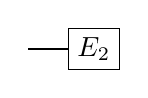
\begin{tikzpicture}
                \node at(1.5,0)[draw, rectangle](ket){$\ket{E_2}$};
                \draw(ket.west)--++(-.5,0);
            \end{tikzpicture}
        }}
        +
        \cdots
    \end{equation*}
    と展開すると、
    \begin{equation*}
        \begin{split}
            &
            \vcenter{\hbox{
                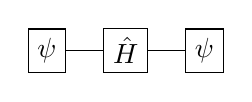
\begin{tikzpicture}
                    \node at(0,0)[draw, rectangle](H){$\hat{H}$};
                    \node at(1.,0)[draw, rectangle](ket){$\ket{\psi}$};
                    \node at(-1.,0)[draw, rectangle](bra){$\bra{\psi}$};
                    \draw(H.west)--(bra.east);
                    \draw(H.east)--(ket.west);
                \end{tikzpicture}
            }}
            \\
            &=
            c_1
            \vcenter{\hbox{
                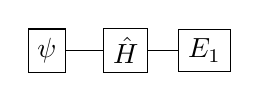
\begin{tikzpicture}
                    \node at(0,0)[draw, rectangle](H){$\hat{H}$};
                    \node at(1.,0)[draw, rectangle](ket){$\ket{E_1}$};
                    \node at(-1.,0)[draw, rectangle](bra){$\bra{\psi}$};
                    \draw(H.west)--(bra.east);
                    \draw(H.east)--(ket.west);
                \end{tikzpicture}
            }}
            +
            c_2
            \vcenter{\hbox{
                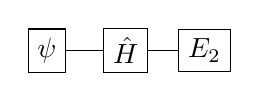
\begin{tikzpicture}
                    \node at(0,0)[draw, rectangle](H){$\hat{H}$};
                    \node at(1.,0)[draw, rectangle](ket){$\ket{E_2}$};
                    \node at(-1.,0)[draw, rectangle](bra){$\bra{\psi}$};
                    \draw(H.west)--(bra.east);
                    \draw(H.east)--(ket.west);
                \end{tikzpicture}
            }}
            +
            \cdots
            \\
            &=
            E_1c_1
            \vcenter{\hbox{
                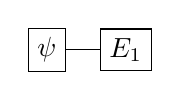
\begin{tikzpicture}
                    \node at(0,0)[draw,rectangle](ket){$\ket{E_1}$};
                    \node at(-1,0)[draw,rectangle](bra){$\bra{\psi}$};
                    \draw(ket.west)--(bra.east);
                \end{tikzpicture}
            }}
            +
            E_2c_2
            \vcenter{\hbox{
                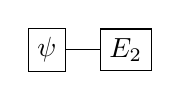
\begin{tikzpicture}
                    \node at(0,0)[draw,rectangle](ket){$\ket{E_2}$};
                    \node at(-1,0)[draw,rectangle](bra){$\bra{\psi}$};
                    \draw(ket.west)--(bra.east);
                \end{tikzpicture}
            }}
            +
            \cdots
        \end{split}
    \end{equation*}
\end{frame}



\section{ひょーげんろん}

\section{ぶんるいもんだい}

\end{document}
